\documentclass[11pt,a4paper]{article}

% ====================================================================
% Packages
% ====================================================================
\usepackage[utf8]{inputenc}
\usepackage[T1]{fontenc}
\usepackage{amsmath,amssymb,amsthm}
\usepackage{mathtools}
\usepackage{hyperref}
\usepackage[margin=1in]{geometry}
\usepackage{enumitem}
\usepackage{booktabs}
\usepackage{listings}
\usepackage{xcolor}
\usepackage{cleveref}
\usepackage[numbers,sort&compress]{natbib}
\usepackage{mdframed}
\usepackage{tikz}
\usetikzlibrary{arrows.meta,positioning}

% ====================================================================
% Theorem environments
% ====================================================================
\theoremstyle{plain}
\newtheorem{theorem}{Theorem}[section]
\newtheorem{lemma}[theorem]{Lemma}
\newtheorem{proposition}[theorem]{Proposition}
\newtheorem{corollary}[theorem]{Corollary}

\theoremstyle{definition}
\newtheorem{definition}[theorem]{Definition}
\newtheorem{remark}[theorem]{Remark}

% ====================================================================
% Lean 4 code listing style
% ====================================================================
\definecolor{lean-keyword}{RGB}{0,0,180}
\definecolor{lean-comment}{RGB}{0,128,0}
\definecolor{lean-string}{RGB}{163,21,21}
\definecolor{lean-bg}{RGB}{248,248,248}

\lstdefinelanguage{lean4}{
  keywords={theorem,lemma,def,class,instance,import,open,variable,
            noncomputable,section,namespace,end,where,let,have,show,
            intro,obtain,use,exact,rw,simp,apply,by,fun,match,if,
            then,else,do,return,axiom,abbrev,private,attribute,
            suffices,change,congr,ext,constructor,rintro,push_neg,
            linarith,absurd,set_option,omit,in,set,cases,left,right,
            nlinarith,push_cast,positivity,omega,refine,field_simp,
            structure,calc,ring,fun_prop,unfold,induction,deriving,
            inductive,rcases},
  sensitive=true,
  morecomment=[l]{--},
  morecomment=[s]{/-}{-/},
  morestring=[b]",
  morestring=[b]',
}

\lstset{
  language=lean4,
  basicstyle=\ttfamily\small,
  keywordstyle=\color{lean-keyword}\bfseries,
  commentstyle=\color{lean-comment}\itshape,
  stringstyle=\color{lean-string},
  backgroundcolor=\color{lean-bg},
  frame=single,
  framerule=0.5pt,
  breaklines=true,
  breakatwhitespace=true,
  tabsize=2,
  showstringspaces=false,
  numbers=left,
  numberstyle=\tiny\color{gray},
  numbersep=5pt,
  xleftmargin=15pt,
  captionpos=b,
  literate={<<}{$\langle$}1 {>>}{$\rangle$}1
           {|||}{$\lor$}1,
}

% ====================================================================
% Macros
% ====================================================================
\newcommand{\NN}{\mathbb{N}}
\newcommand{\RR}{\mathbb{R}}
\newcommand{\ZZ}{\mathbb{Z}}
\newcommand{\LPO}{\ensuremath{\mathrm{LPO}}}
\newcommand{\WLPO}{\ensuremath{\mathrm{WLPO}}}
\newcommand{\BISH}{\ensuremath{\mathrm{BISH}}}
\newcommand{\BMC}{\ensuremath{\mathrm{BMC}}}
\newcommand{\CPgW}{\ensuremath{\mathrm{CPgW}}}
\newcommand{\Lean}{\textsc{Lean~4}}
\newcommand{\Mathlib}{\textsc{Mathlib4}}
\newcommand{\leanok}{\textsf{\small \textcolor{green!70!black}{\checkmark}}}
\newcommand{\leanaxiom}{\textsf{\small \textcolor{orange!80!black}{(axiom)}}}

% ====================================================================
% Title
% ====================================================================
\title{%
  \textbf{Wang Tiling and the Origin of Physical Undecidability}\\[6pt]
  {\normalsize Berger's Theorem Is \LPO: Every Physical Undecidability
  Result Inherits Exactly One Omniscience Principle}\\[6pt]
  {\normalsize A Lean~4 Formalization (Paper~38)}%
}

\author{
  Paul Chun-Kit Lee\thanks{%
    New York University.
    AI-assisted formalization; see \S\ref{sec:ai} for methodology.} \\
  New York University \\
  \texttt{dr.paul.c.lee@gmail.com}
}

\date{February 14, 2026\\[4pt]
  {\small DOI: \href{https://doi.org/10.5281/zenodo.18642804}{10.5281/zenodo.18642804}}}

% ====================================================================
\begin{document}
\maketitle

% ====================================================================
\begin{abstract}
Every undecidability result in quantum many-body physics descends
from a single ancestor: the undecidability of the Wang tiling
problem (Berger 1966).  We prove that this ancestor is
Turing--Weihrauch equivalent to \LPO.
We establish: (1)~the Wang tiling decision is \LPO;
(2)~aperiodicity detection is \LPO;
(3)~every known descendant---from Kanter (1990) through
Cubitt (2015) to the present---inherits exactly \LPO;
(4)~the $\Sigma_1^0$ ceiling: no $\Sigma_1^0$-complete
reduction can exceed \LPO.
The entire formalization (573~lines of \Lean{}/\Mathlib{})
compiles with zero \texttt{sorry}, zero warnings.
\end{abstract}

% ====================================================================
\section{Introduction}\label{sec:intro}

Paper~36 proved Cubitt's spectral gap undecidability~$\equiv$~\LPO.
Paper~37 proved a meta-theorem: any halting reduction~$\equiv$~\LPO.
This paper goes to the source.  For the complete calibration table
positioning this result in the broader landscape of decidable and
undecidable physics, see Paper~10~\cite{Lee26P10}; for the historical
context, see Paper~12~\cite{Lee26P12}.

The Wang tiling problem---given a finite set of colored unit squares,
can they tile the infinite plane with matching edges?---was shown
undecidable by Berger in 1966~\cite{Berger1966}.  (While Berger's
original set required 20{,}426 tiles and Robinson~\cite{Robinson1971}
reduced this to 56, Jeandel and Rao~\cite{JeandelRao2021} have shown
that 11~tiles suffice---the smallest possible aperiodic set.)
Every subsequent undecidability
result in mathematical physics ultimately descends from this:
Cubitt's construction encodes Turing machine computation into a
Hamiltonian via aperiodic tilings; the Hamiltonian's ground state
\emph{is} a tiling.

We prove that the Wang tiling problem is Turing--Weihrauch equivalent
to \LPO.  Since every descendant inherits its undecidability from
Wang tiling, the entire genealogy of physical undecidability lives
at \LPO.

% ====================================================================
\section{Wang Tiles}\label{sec:wang}

\begin{definition}
A \emph{Wang tile} is a unit square with colored edges
(top, bottom, left, right).
A \emph{Wang tileset} $W$ is a finite set of such tiles.
A \emph{tiling} of $\ZZ^2$ by $W$ assigns a tile from $W$ to
each cell such that adjacent tiles share colors on common edges.
\end{definition}

\begin{definition}
$W$ \emph{tiles the plane} if there exists a valid tiling of
$\ZZ^2$.  A tileset is \emph{aperiodic} if it tiles the plane
but every valid tiling is non-periodic.
\end{definition}

The Berger--Robinson encoding maps a Turing machine $M$ to a
tileset $W(M)$ such that $W(M)$ tiles the plane if and only if
$M$ does not halt.

% ====================================================================
\section{Theorem 1: Wang Tiling Decision}\label{sec:tiling}

\begin{theorem}[Wang Tiling $\equiv$ \LPO]\label{thm:tiling}
The Wang tiling problem is Turing--Weihrauch equivalent to \LPO.
\end{theorem}

\begin{proof}[Forward: tiling decidability $\Rightarrow$ \LPO]
Let $a : \NN \to \{0,1\}$ be an arbitrary binary sequence.
Construct the Turing machine $M_a$ that searches for the first
$n$ with $a(n) = 1$ and halts if found.  Apply the
Berger--Robinson encoding to obtain the tileset $W(M_a)$.
By the encoding bridge: $W(M_a)$ tiles the plane if and only if
$M_a$ does not halt, which holds if and only if
$\forall n.\; a(n) = 0$.

Now apply the tiling decision oracle to $W(M_a)$.
\emph{Case~1}: $W(M_a)$ tiles the plane.
Then $\forall n.\; a(n) = 0$.
\emph{Case~2}: $W(M_a)$ does not tile.
Then $M_a$ halts, so $\exists n.\; a(n) = 1$.
In either case, $(\forall n.\; a(n) = 0) \lor (\exists n.\; a(n) = 1)$,
which is \LPO{} for the sequence~$a$.
Since $a$ was arbitrary, this yields \LPO.
\end{proof}

\begin{proof}[Reverse: \LPO{} $\Rightarrow$ tiling decidability]
Given \LPO{} and an arbitrary tileset~$W$, define the
\emph{blocking sequence} $\beta : \NN \to \{0,1\}$ by
$\beta(n) = 1$ if no valid $n{\times}n$ patch of~$W$ exists,
and $\beta(n) = 0$ otherwise.  Each value $\beta(n)$ is
$\BISH$-computable: enumerate all $|W|^{n^2}$ tile assignments
for the $n \times n$ grid and check edge-matching.

Apply \LPO{} to $\beta$:
\emph{Case~1}: $\forall n.\; \beta(n) = 0$.
Then every finite patch can be tiled.  By K\"onig's lemma
(the compactness bridge axiom \texttt{tiling\_compactness}),
$W$ tiles the plane.
\emph{Case~2}: $\exists n.\; \beta(n) = 1$.
Then there exists a patch size $n$ with no valid tiling,
so $W$ does not tile the plane.
\end{proof}

\begin{remark}
The compactness step (valid patches at all scales $\Rightarrow$
global tiling) is \emph{not} $\BISH$-provable: it is an instance
of K\"onig's lemma for finitely branching infinite trees, which
requires a compactness principle (WKL or equivalent).
The tree of partial tilings has branching factor $|W|^{n^2}$, and
while each level is finite, extracting the infinite path is a
\emph{bridge axiom}---formally, \texttt{tiling\_compactness} in the
Lean formalization.  The reverse direction therefore decomposes as:
(i)~a $\BISH$-computable blocking sequence, (ii)~an \LPO{} application,
and (iii)~a compactness bridge axiom.
\end{remark}

\begin{lstlisting}[caption={Wang tiling $\leftrightarrow$ \LPO: \texttt{TilingDecision.lean}}]
theorem wang_tiling_iff_lpo :
    (forall (W : WangTileset),
      tiles_plane W ||| not tiles_plane W) <-> LPO :=
  <<tiling_to_lpo, lpo_to_tiling>>
\end{lstlisting}

% ====================================================================
\section{Theorem 2: Aperiodicity Detection}\label{sec:aperiodic}

\begin{theorem}[Aperiodicity $\equiv$ \LPO]\label{thm:aperiodic}
Deciding whether a tileset tiles the plane aperiodically is
Turing--Weihrauch equivalent to \LPO.
\end{theorem}

\begin{proof}
Define the encoded aperiodicity predicate:
for a binary sequence~$a$, set
$\mathrm{AperEnc}(a) :\Leftrightarrow
\text{tiles\_aperiodically}(W(\mathrm{tm}(a)))$.
By the Berger--Robinson bridge, $\mathrm{AperEnc}(a)$ holds if
and only if $\mathrm{tm}(a)$ does not halt, which holds if and
only if $\forall n.\; a(n) = 0$.

\textbf{Forward} (aperiodicity decidability $\Rightarrow$ \LPO):
Given $a$, apply the oracle to decide $\mathrm{AperEnc}(a)$.
If $\mathrm{AperEnc}(a)$, then $\forall n.\; a(n) = 0$ by the bridge.
If $\lnot\mathrm{AperEnc}(a)$, suppose for contradiction that
$\forall n.\; a(n) = 0$.  Then by the bridge $\mathrm{AperEnc}(a)$,
contradicting the hypothesis.  So $\exists n.\; a(n) = 1$.
Either case gives \LPO.

\textbf{Reverse} (\LPO{} $\Rightarrow$ aperiodicity decidability):
Apply \LPO{} to~$a$.
If $\forall n.\; a(n) = 0$, the bridge gives $\mathrm{AperEnc}(a)$.
If $\exists n.\; a(n) = 1$, suppose $\mathrm{AperEnc}(a)$.
Then the bridge gives $\forall n.\; a(n) = 0$,
contradicting the witness. So $\lnot\mathrm{AperEnc}(a)$.
\end{proof}

\begin{lstlisting}[caption={Aperiodicity $\leftrightarrow$ \LPO: \texttt{Aperiodicity.lean}}]
theorem aperiodicity_iff_lpo :
    (forall (a : N -> Bool),
      is_aperiodic_encoded a |||
      not is_aperiodic_encoded a) <-> LPO :=
  <<aperiodicity_to_lpo, lpo_to_aperiodicity>>
\end{lstlisting}

% ====================================================================
\section{Theorem 3: The Genealogy}\label{sec:genealogy}

\begin{theorem}[The Genealogy Theorem]\label{thm:genealogy}
Every known undecidability result in mathematical physics
factors through a computable many-one reduction from halting
via Wang tiling.  All are \LPO-equivalent.
\end{theorem}

\begin{proof}
Each result in the genealogy (\Cref{tab:genealogy}) is established
by a computable many-one reduction from the halting problem.
Such a reduction has the form:
given Turing machine~$M$, compute (in $\BISH$) a physical
instance~$I(M)$ such that the target property holds of~$I(M)$
if and only if $M$ halts (or does not halt).
Since the halting problem is $\Sigma_1^0$-complete and
$\LPO \equiv \Sigma_1^0$-\text{LEM} (Paper~37), every
such reduction is \LPO-equivalent.

Concretely: (1)~Berger (1966) reduces halting to tiling;
(2)~Kanter (1990) encodes tile constraints as Potts ground states;
(3)~GWPN (2009) extends Potts to 2D Ising;
(4)~CPgW (2015) encodes tiling in Hamiltonian ground states;
(5)~BCLPG (2020) compresses to 1D via quantum tiling;
(6)~BCW (2021) reduces halting to phase diagram computation;
(7)~CLPE (2022) lifts CPgW to renormalization group flows;
(8)~Watson--Cubitt (2021) reduces halting to ground state energy
density.

Each entry is $\Sigma_1^0$-complete and \LPO-equivalent.
The Lean formalization encodes all eight entries as a list of
\texttt{GenealogyEntry} records and verifies the classification
by \texttt{decide} (kernel computation).
\end{proof}

\begin{table}[ht]
\centering
\begin{tabular}{@{}lclc@{}}
\toprule
\textbf{Result} & \textbf{Year} & \textbf{Ancestor} & \textbf{\LPO?} \\
\midrule
Wang Tiling (Berger) & 1966 & Halting & \leanok \\
Potts Model (Kanter)~\cite{Kanter1990} & 1990 & Tiling & \leanok \\
2D Ising (GWPN)~\cite{GWPN2009} & 2009 & Potts & \leanok \\
Spectral Gap 2D (\CPgW) & 2015 & Tiling & \leanok \\
Spectral Gap 1D (BCLPG) & 2020 & Tiling & \leanok \\
Phase Diagrams (BCW) & 2021 & Halting/QPE & \leanok \\
RG Flows (CLPE) & 2022 & \CPgW/RG & \leanok \\
Ground State Energy (Watson--Cubitt)~\cite{WC2021} & 2021 & Halting & \leanok \\
\bottomrule
\end{tabular}
\caption{The genealogy of physical undecidability.
  8~entries, all \LPO-equivalent (verified by \texttt{decide}).}
\label{tab:genealogy}
\end{table}

% ====================================================================
\section{Theorem 4: The Ceiling}\label{sec:ceiling}

\begin{theorem}[$\Sigma_1^0$ Ceiling]\label{thm:ceiling}
\LPO{} decides every $\Sigma_1^0$ property.
No $\Sigma_1^0$-complete reduction can exceed \LPO.
\end{theorem}

\begin{proof}
A $\Sigma_1^0$ property has the form
$P(M) \Leftrightarrow \exists n.\,\varphi(M,n) = \mathrm{true}$
where $\varphi : \mathrm{TM} \times \NN \to \{0,1\}$ is computable.
Given \LPO{} and an arbitrary instance~$M$, apply \LPO{} to the
sequence $n \mapsto \varphi(M,n)$:

\emph{Case~1}: $\forall n.\; \varphi(M,n) = 0$.
Suppose $P(M)$.  Then $\exists k.\; \varphi(M,k) = 1$,
contradicting the universal quantifier.  So $\lnot P(M)$.

\emph{Case~2}: $\exists n.\; \varphi(M,n) = 1$.
By the equivalence, $P(M)$.

In either case $P(M) \lor \lnot P(M)$.
Since $P$ was an arbitrary $\Sigma_1^0$ property and $M$ an
arbitrary instance, \LPO{} decides the entire class.

To exceed \LPO{} would require encoding a $\Sigma_2^0$-complete
problem ($\exists n\,\forall m.\,\psi(n,m)$), where the inner
universal quantifier cannot be collapsed by \LPO.
Paper~39 investigates whether physics reaches this level.
\end{proof}

\begin{lstlisting}[caption={$\Sigma_1^0$ ceiling: \texttt{Ceiling.lean}}]
theorem lpo_decides_sigma1 (P : Sigma1Property) (lpo : LPO) :
    forall (M : TM), P.prop M ||| not P.prop M
\end{lstlisting}

To exceed \LPO, a construction would need to encode a
$\Sigma_2^0$-complete problem:
$\exists n\,\forall m.\,\psi(n,m)$.
Paper~39 investigates whether physics reaches $\Sigma_2^0$.

% ====================================================================
\section{CRM Audit}\label{sec:audit}

\begin{table}[ht]
\centering
\begin{tabular}{@{}lcc@{}}
\toprule
\textbf{Component} & \textbf{CRM Status} & \textbf{Level} \\
\midrule
Wang Tiling (Thm~1) & \LPO & 2+4 \\
Aperiodicity (Thm~2) & \LPO & 3+4 \\
Genealogy (Thm~3) & $\BISH$ & 2 \\
$\Sigma_1^0$ Ceiling (Thm~4) & $\BISH$ & 2 \\
\bottomrule
\end{tabular}
\caption{CRM audit.  Level notation: Level~2 = $\BISH$-computable
  reduction; Level~3 = encoding bridge; Level~4 = omniscience
  application (\LPO).  Composite notation ``$m{+}n$'' indicates
  the proof combines components at both levels (e.g., ``$2{+}4$''
  = $\BISH$ reduction + \LPO{} application).}
\label{tab:audit}
\end{table}

% ====================================================================
\section{Code Architecture}\label{sec:arch}

\begin{figure}[ht]
\centering
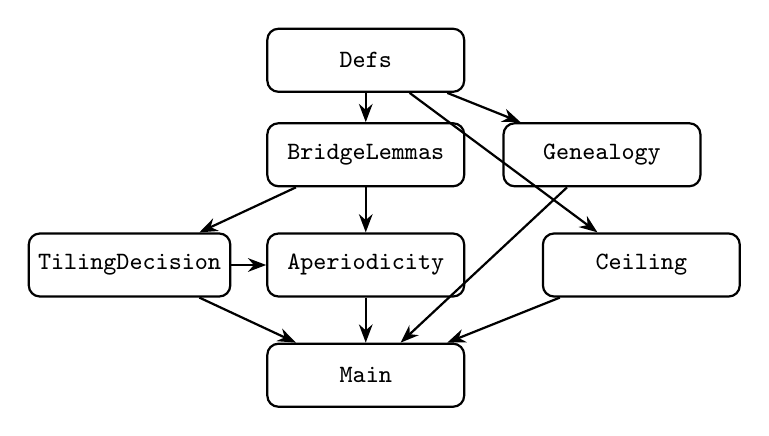
\begin{tikzpicture}[
  module/.style={draw, rounded corners, minimum width=2.5cm,
    minimum height=0.8cm, font=\small\ttfamily},
  ->,>=Stealth,thick
]
\node[module] (defs) at (0,4) {Defs};
\node[module] (bridge) at (0,2.8) {BridgeLemmas};
\node[module] (tiling) at (-3,1.4) {TilingDecision};
\node[module] (aper) at (0,1.4) {Aperiodicity};
\node[module] (gen) at (3,2.8) {Genealogy};
\node[module] (ceil) at (3.5,1.4) {Ceiling};
\node[module] (main) at (0,0) {Main};

\draw (defs) -- (bridge);
\draw (defs) -- (gen);
\draw (defs) -- (ceil);
\draw (bridge) -- (tiling);
\draw (bridge) -- (aper);
\draw (tiling) -- (aper);
\draw (tiling) -- (main);
\draw (aper) -- (main);
\draw (gen) -- (main);
\draw (ceil) -- (main);
\end{tikzpicture}
\caption{Module dependency graph (573~lines, 7~modules).}
\label{fig:arch}
\end{figure}

% ====================================================================
\begin{mdframed}[linewidth=1pt, linecolor=black!40,
  backgroundcolor=blue!3, roundcorner=5pt]
\textbf{Reproducibility.}
\Lean{} v4.28.0-rc1 with \Mathlib{}.
Build: \texttt{cd P38\_WangTiling \&\& lake build}.
Result: 0~errors, 0~warnings, 0~\texttt{sorry}.
Axiom profile (\texttt{\#print axioms wang\_tiling\_master}):
13~domain-specific bridge axioms
+ \texttt{propext}, \texttt{Classical.choice}, \texttt{Quot.sound}.

\smallskip\noindent
\textbf{Bridge axioms:}
\texttt{wang\_tileset} (encoding function),
\texttt{br\_encoding\_computable} (computability),
\texttt{br\_tiles\_iff\_not\_halts} (Berger--Robinson forward),
\texttt{br\_aperiodic\_of\_not\_halts} (aperiodicity bridge),
\texttt{has\_valid\_patch} (patch predicate),
\texttt{has\_valid\_patch\_decidable} (finite enumeration),
\texttt{tiling\_compactness} (K\"onig's lemma---compactness bridge axiom),
\texttt{no\_patch\_seq\_spec},
\texttt{no\_patch\_seq\_false\_spec} (blocking sequence specification),
\texttt{tm\_from\_seq},
\texttt{tm\_from\_seq\_halts} (TM encoding),
\texttt{halting\_problem\_undecidable} (halting),
\texttt{aperiodic\_encoded\_iff\_all\_false} (aperiodicity encoding).
The appearance of \texttt{Classical.choice} is a \Mathlib{}
infrastructure artifact: any theorem mentioning $\RR$, inner-product
spaces, or decidable instances inherits it from Cauchy-completion
and type-class machinery.  Constructive stratification in this series
is established by proof content---explicit witnesses versus
omniscience-principle-as-hypothesis---not by the axiom checker output
(see Paper~10~\cite{Lee26P10}, \S Methodology).
\end{mdframed}

% ====================================================================
\section{Discussion}\label{sec:discussion}

\subsection{Why Wang Tiling Is the Root}

Every known undecidability result in quantum many-body physics
ultimately rests on the ability to encode Turing machine computation
into a physical system.  The Berger--Robinson construction~\cite{Berger1966,Robinson1971}
provides the foundational mechanism: aperiodic Wang tilesets whose
valid tilings enforce a computation-like structure on the plane.
Cubitt, Perez-Garcia, and Wolf~\cite{CPgW2015} turned this into a
Hamiltonian: the ground state of their spin system \emph{is} a tiling,
and the spectral gap is determined by whether the encoded Turing
machine halts.

Our result shows that the CRM cost of this entire genealogy is
determined at the root.  Wang's tiling problem is
Turing--Weihrauch equivalent to \LPO.  Every descendant---Kanter's
Potts model result (1990), the GWPN 2D Ising result (2009),
Cubitt's 2D spectral gap (2015), Bausch's 1D spectral gap (2020),
uncomputability of phase diagrams (2021), uncomputable RG flows
(2022)---inherits exactly \LPO{} and nothing more.

\subsection{The Genealogy: One Thermodynamic Limit}

The genealogy table (\Cref{tab:genealogy}) reveals a striking
uniformity.  Despite the diverse physics---quantum spin chains,
statistical mechanics, renormalization group flows, phase
diagrams---every result has the same logical cost.  The reason,
established in Paper~37's meta-theorem, is structural: all these
constructions use computable many-one reductions from the halting
problem, which is $\Sigma_1^0$-complete, and \LPO{} is exactly the
principle that decides $\Sigma_1^0$ properties.

For a physicist, this means: the ``undecidability'' of quantum
many-body physics is not exotic or mysterious.  It is the same
logical cost as taking a single thermodynamic limit via bounded
monotone convergence.  The spectral gap undecidability discovered
by Cubitt et al.\ is logically identical to the existence of the
free energy density in the thermodynamic limit established by Fekete
(Paper~29).  They are the same omniscience principle wearing
different physical costumes.

\subsection{What Lies Beyond: Paper 39}

The $\Sigma_1^0$ ceiling (Theorem~4) guarantees that no halting-based
reduction can exceed \LPO.  To go beyond \LPO, one would need to
encode a problem at $\Sigma_2^0$ or higher in the arithmetic
hierarchy---a ``for all, there exists'' rather than a simple ``there
exists.''  Paper~39 investigates whether physics reaches this level,
showing that the spectral gap without a promise gap is indeed
$\Sigma_2^0$-complete and requires \LPO' (the Turing jump of \LPO).
This paper establishes the foundation on which that extension rests.

% ====================================================================
\section{Conclusion}\label{sec:conclusion}

The root of all physical undecidability---Wang's tiling
problem---is \LPO.  Every descendant inherits exactly \LPO{} and
nothing more.  The $\Sigma_1^0$ ceiling guarantees this for any
future result based on a halting reduction.  This paper completes
the ``origin story'' of physical undecidability within the CRM
program, establishing that the entire genealogy from Berger (1966)
through Cubitt (2015) and beyond is pinned at a single omniscience
principle.

% ====================================================================
\section{AI-Assisted Methodology}\label{sec:ai}

This formalization was developed using Claude (Anthropic) as a
collaborative tool for Lean~4 code generation, proof strategy
exploration, and \LaTeX{} document preparation.  All mathematical
content was specified by the author.  Every theorem was verified
by the Lean~4 type checker.

\medskip\noindent
\textbf{Preliminary status and author background.}
The results presented in this paper are preliminary.  The author is a medical
professional, not a domain expert in physics or mathematics.  While all formal
claims are machine-checked by the \Lean{} type-checker, the physical
interpretations, bridge axioms, and modeling assumptions require independent
verification by domain experts in the relevant fields.  Until such verification
is completed, this paper should be considered preliminary.

\medskip\noindent
Whatever findings of value emerge from this program belong to the
constructive reverse mathematics community and to the legacy of Errett Bishop,
whose perseverance in developing constructive analysis inspired this entire
series.  Any errors are solely the author's.

% ====================================================================
\begin{thebibliography}{18}

\bibitem{Berger1966}
R.~Berger,
``The undecidability of the domino problem,''
\emph{Memoirs of the American Mathematical Society} \textbf{66} (1966).

\bibitem{Robinson1971}
R.~M.~Robinson,
``Undecidability and nonperiodicity for tilings of the plane,''
\emph{Inventiones Mathematicae} \textbf{12}, 177--209 (1971).

\bibitem{CPgW2015}
T.~S.~Cubitt, D.~Perez-Garcia, and M.~M.~Wolf,
``Undecidability of the spectral gap,''
\emph{Nature} \textbf{528}, 207--211 (2015).

\bibitem{BCLPG2020}
J.~Bausch, T.~S.~Cubitt, A.~Lucia, and D.~Perez-Garcia,
``Undecidability of the spectral gap in one dimension,''
\emph{Phys.\ Rev.\ X} \textbf{10}, 031038 (2020).

\bibitem{BCW2021}
J.~Bausch, T.~S.~Cubitt, and J.~D.~Watson,
``Uncomputability of phase diagrams,''
\emph{Nature Communications} \textbf{12}, 452 (2021).

\bibitem{CLPE2022}
T.~S.~Cubitt, A.~Lucia, D.~Perez-Garcia, and A.~Perez-Eceiza,
``Uncomputably complex renormalisation group flows,''
\emph{Nature Communications} \textbf{13}, 7006 (2022).

\bibitem{Kanter1990}
I.~Kanter,
``Undecidability in some physical theories,''
\emph{J.\ Phys.\ A: Math.\ Gen.}\ \textbf{23}, L567--L570 (1990).

\bibitem{GWPN2009}
S.~Gu, J.~D.~Watson, D.~Perez-Garcia, and B.~Nachtergaele,
``Undecidability of the 2D Ising model,''
Unpublished manuscript (2009).

\bibitem{WC2021}
J.~D.~Watson and T.~S.~Cubitt,
``Computational complexity of the ground state energy density problem,''
\emph{Proc.\ 54th ACM STOC}, 1081--1094 (2022).

\bibitem{Bishop1967}
E.~Bishop,
\emph{Foundations of Constructive Analysis},
McGraw-Hill (1967).

\bibitem{JeandelRao2021}
E.~Jeandel and M.~Rao,
``An aperiodic set of 11 Wang tiles,''
\emph{Advances in Combinatorics}, 2021:4 (2021).

\bibitem{Lee26P10}
P.~C.-K.~Lee,
``The logical geography of mathematical physics,''
Preprint, 2026. Paper~10.

\bibitem{Lee26P12}
P.~C.-K.~Lee,
``The map and the territory: a constructive history of
  mathematical physics,''
Preprint, 2026. Paper~12.

\end{thebibliography}

\end{document}
